\subsection{Lo-fi prototyping}\label{subsec:lo-fi-prototyping}

After the early prototyping phase, the group started to create a low-fidelity prototype~\cite{hi-lo-fidelity}.
This was done during a hackathon week, where the group had the opportunity to work on the prototypes together with
other groups.
Therefore, the group got a lot of feedback from other groups, which helped to improve the design.
The specific feedback is discussed in Section~\ref{sec:evaluation}.

This design, which can be seen in Figure~\ref{fig:lofi-prototype}, is made out of pen and paper.
It is made to be modular, which means that different charts and options can be attached or removed.
This encourages interactivity when testing the prototype.
The design focuses on a single chart at a time with an option to filter
the data using the calendar view on the bottom.
The charts can be switched between using the buttons on either side of the chart.
The calendar on the bottom can be clicked on to filter data for a specific time period.
The examples in the figure include:

\begin{itemize}
    \item The login page as seen in Figure~\ref{subfig:lofi-login}.
    This is the page where the user attempts to log in to the application.
    \item The upload page as seen in Figure~\ref{subfig:lofi-upload}.
    This is where the user attempts to upload a CSV file with order data.
    \item The bar chart and heatmap as seen in Figure~\ref{subfig:lofi-bar} and~\ref{subfig:lofi-heatmap} respectively.
    These are both components that show the user some data.
\end{itemize}

\begin{figure}[H]
    \centering
    \begin{subfigure}{.49\textwidth}
        \centering
        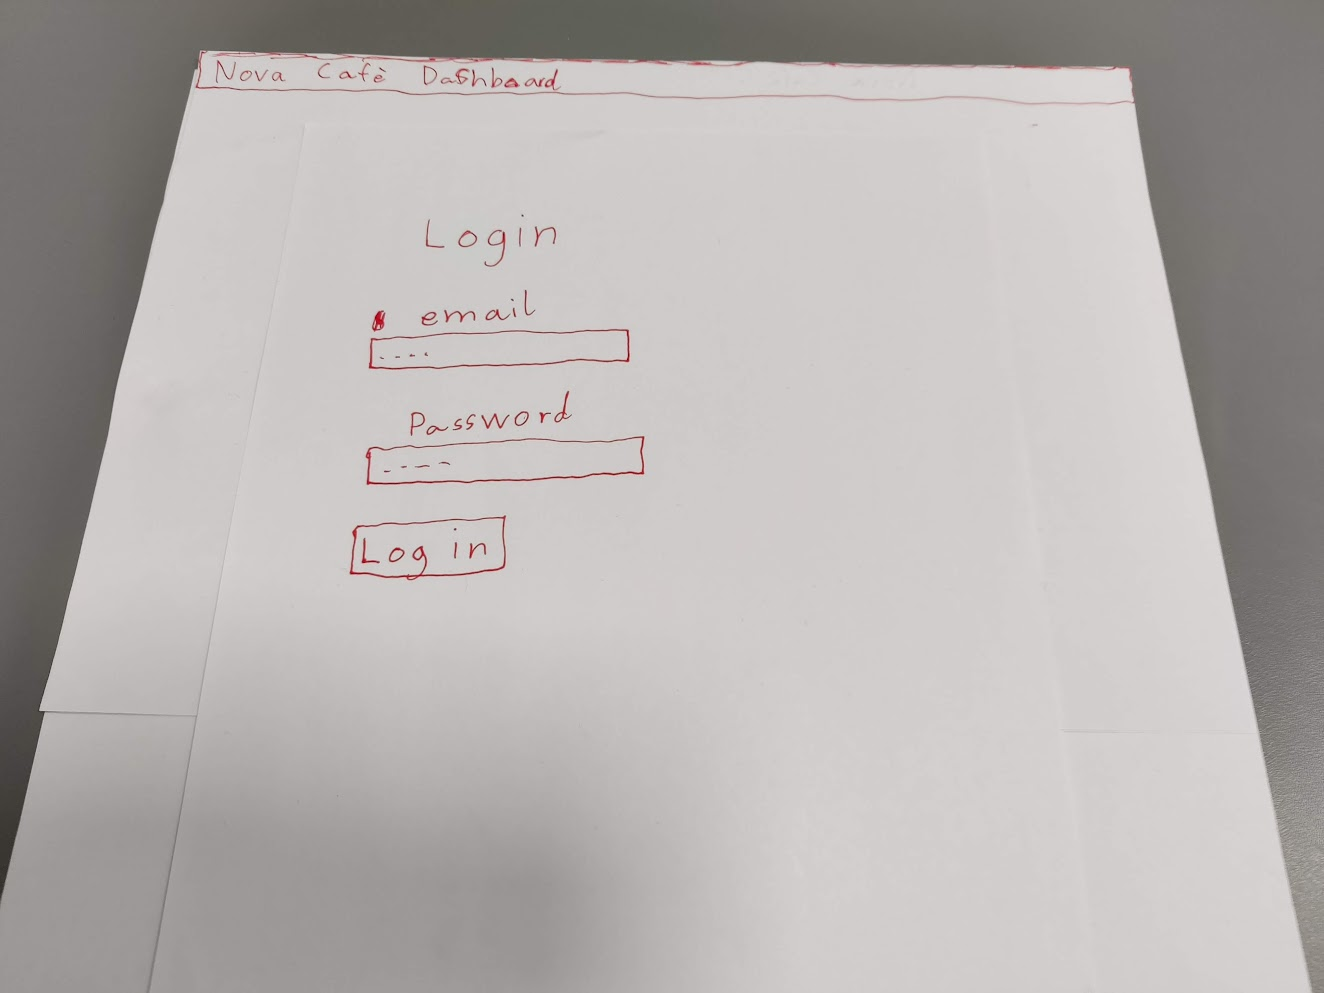
\includegraphics[width=\linewidth]{design-lofi-login}
        \caption{Login page.
        }\label{subfig:lofi-login}
    \end{subfigure}
    \begin{subfigure}{.49\textwidth}
        \centering
        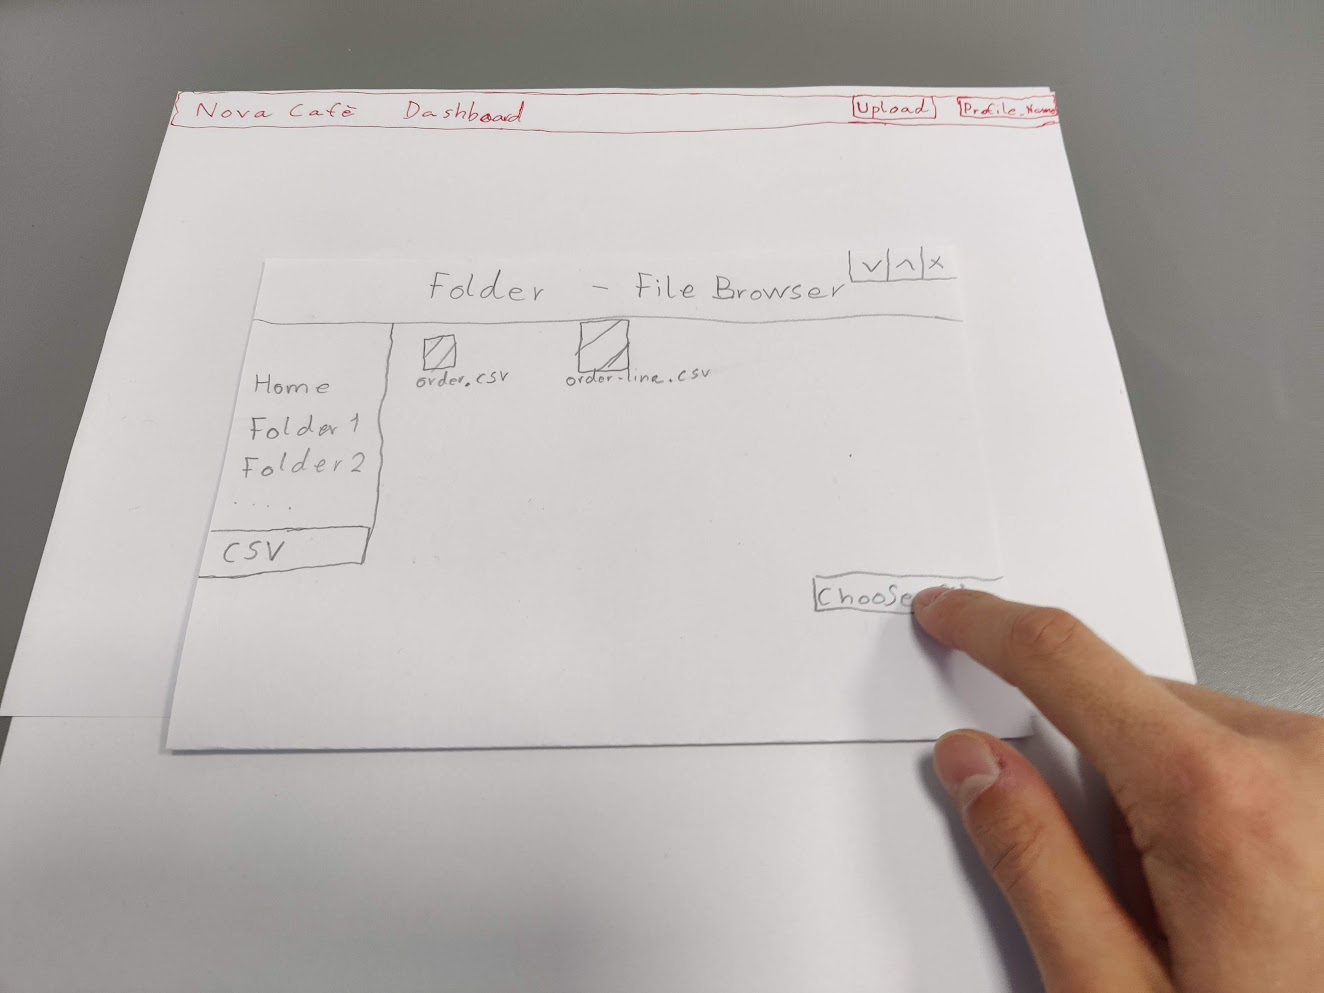
\includegraphics[width=\linewidth]{design-lofi-upload}
        \caption{Upload page.
        }\label{subfig:lofi-upload}
    \end{subfigure}
    \par\medskip
    \begin{subfigure}{.49\textwidth}
        \centering
        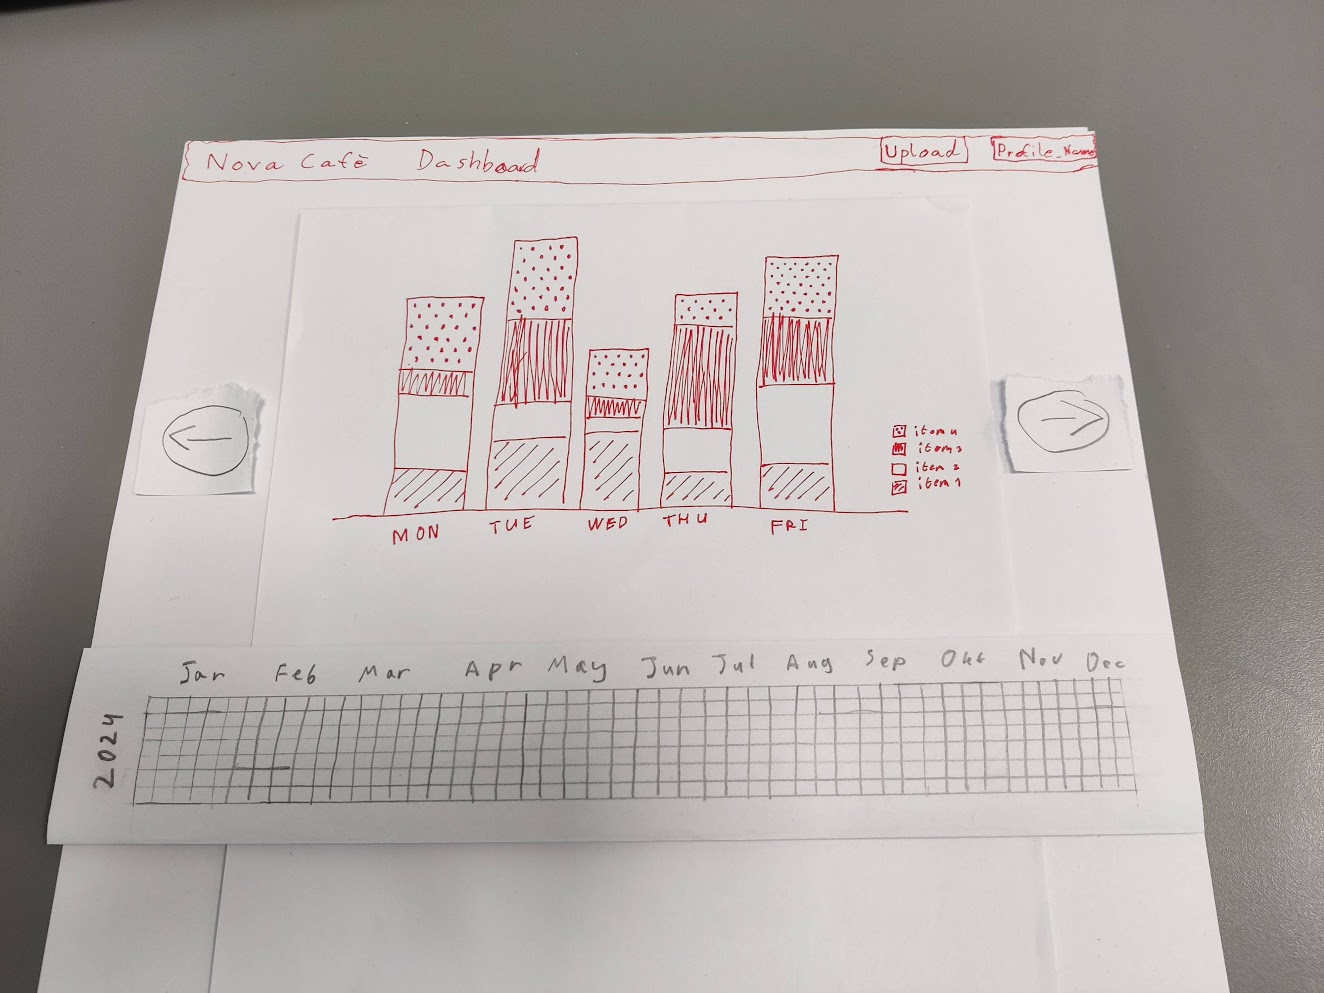
\includegraphics[width=\linewidth]{design-lofi-bar}
        \caption{Bar chart.
        }\label{subfig:lofi-bar}
    \end{subfigure}
    \begin{subfigure}{.49\textwidth}
        \centering
        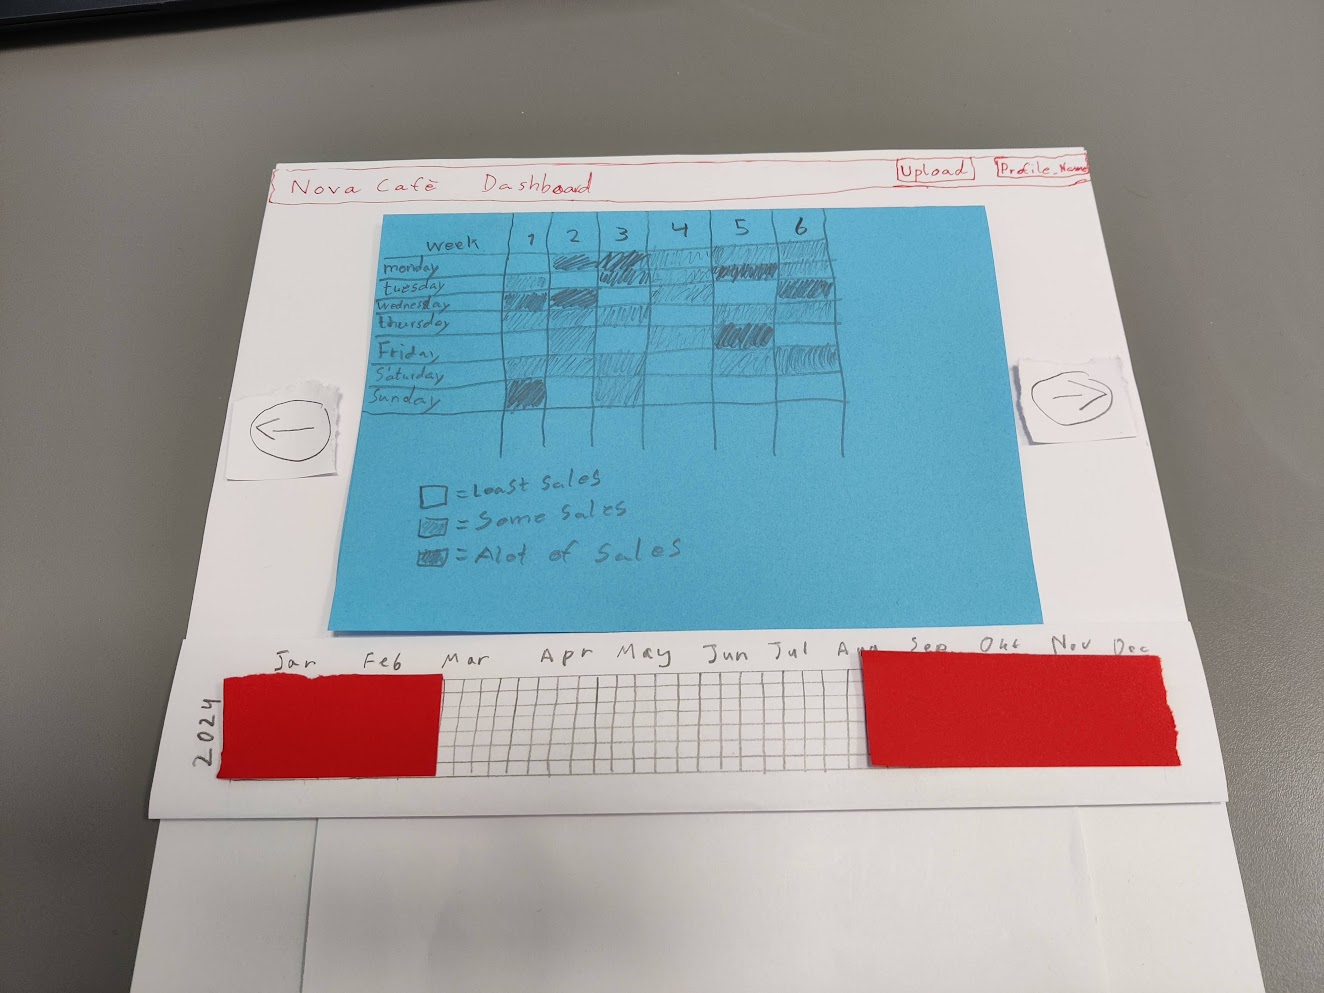
\includegraphics[width=\linewidth]{design-lofi-heatmap}
        \caption{Heatmap.
        }\label{subfig:lofi-heatmap}
    \end{subfigure}
    \caption{Lo-fi prototypes of four components.
    }\label{fig:lofi-prototype}
\end{figure}
